\section{Presentación}
Soy \emph{Ingeniero Electrónico} del ITBA, recibido recientemente de \emph{Especialista
en Sistemas Embebidos} y cursando una \emph{Maestría en Sistemas Embebidos} de la UBA. \\
Desarrollé mi carrera trabajando en el área de desarrollo de producto de varias
empresas nacionales y en el área de investigación en instituciones estatales.\\
Estuve a cargo de un estudio de ingeniería electrónica ofreciendo servicios de
diseño y producción electrónica y actualmente trabajo como desarrollador
electrónico freelance.\\ %con posibilidad de emitir facturas 'A' y 'B'.\\ mepa que no da esto
Trabajo diariamente diseñando equipos electrónicos embebidos ejecutando tareas como: \\
\cvlistitem{Toma de requerimientos y planificación de los test de aceptación de hard y soft.}
\cvlistitem{Diseño de esquemáticos, PCB, simulaciones, montaje, modelado 3D y mecanizados.}
\cvlistitem{Codificación para tiempo real en C/C++ en bare metal o sobre RTOS. }
\cvlistitem{Codificación de scripts en Bash y Python sobre Linux y Linux embebido.}
\cvlistitem{Codificación y ejecución de los test unitarios y manejo de herramientas de integración continua.}
\cvlistitem{Armado y puesta en marcha de prototipos y documentación para la Línea de montaje.}
Soy muy pragmático, comprometido y disfruto resolver los problemas complejos de
modo creativo intercambiando ideas con mis pares. Prefiero los desarrollos
down-top utilizando conceptos ágiles para mantener el producto funcional desde
el inicio.\\
Cuento con un laboratorio de desarrollo de electrónica, mostrado en la figura \ref{fig:ofi_dci} y en el \href{\linkofidci}{video}, con herramientas tales como: \\
\cvlistitem{Línea de montaje de placas SMD y TH, stencil de pasta, pick and place, horno de refusión y batea.}
\cvlistitem{Herramientas de reworking y soldadura manual}
\cvlistitem{Stock de materiales SMD y TH de uso corriente y específicos.}
\cvlistitem{Centro de mecanizado CNC.}
\cvlistitem{Máquina para corte y grabado laser.}
\cvlistitem{Varias maquinas para impresión 3D.}
\cvlistitem{Generadores, Osciloscopios e Instrumental avanzado para medición y diagnóstico.}
\cvlistitem{Herramientas electrónicas para desarrollo de firmware.}
Estas herramientas, mi experiencia, capacidad técnica y frecuente actualización académica me
permiten desenvolverme en la mayoría de las instancias del desarrollo de un
equipo electrónico embebido profesional.\\
Sigue los links para ver videos, pdf's e información detallada de cada sección.\\
Se puede acceder al CV mas reciente \href{\linkgithubcvpdf}{aquí}.\\
  \begin{figure}
      \begin{center}
         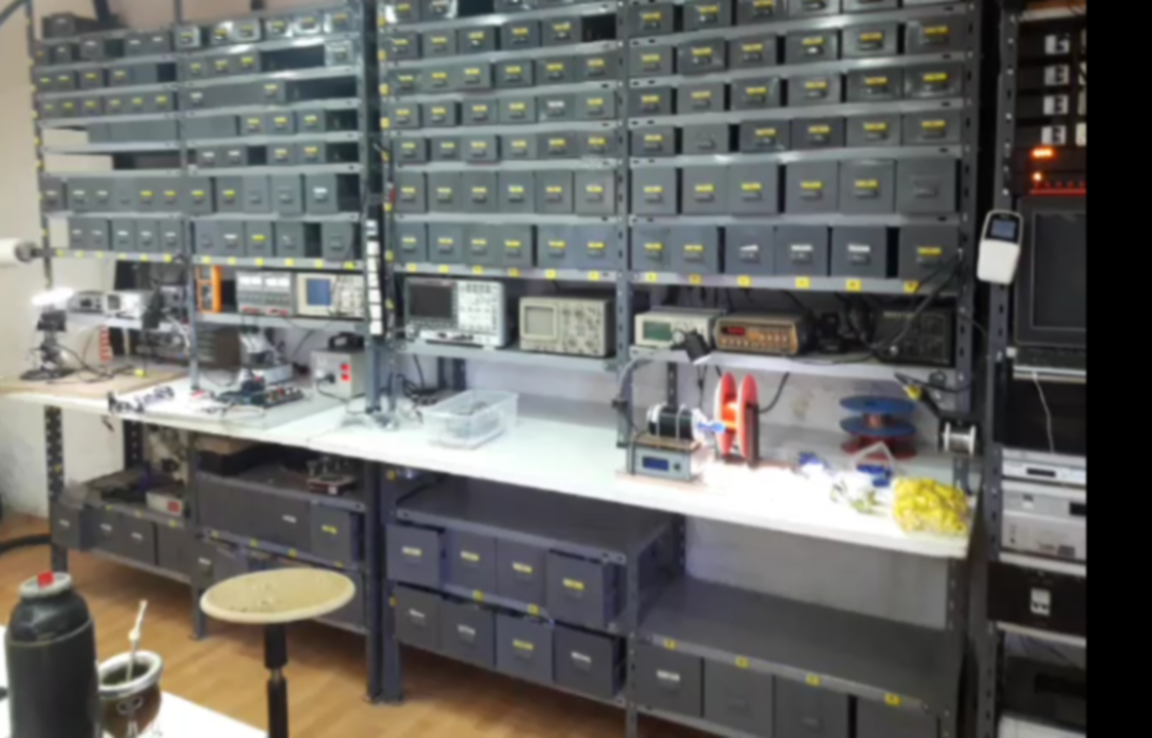
\includegraphics[width=0.3\textwidth]{ofi_dci1.png}
         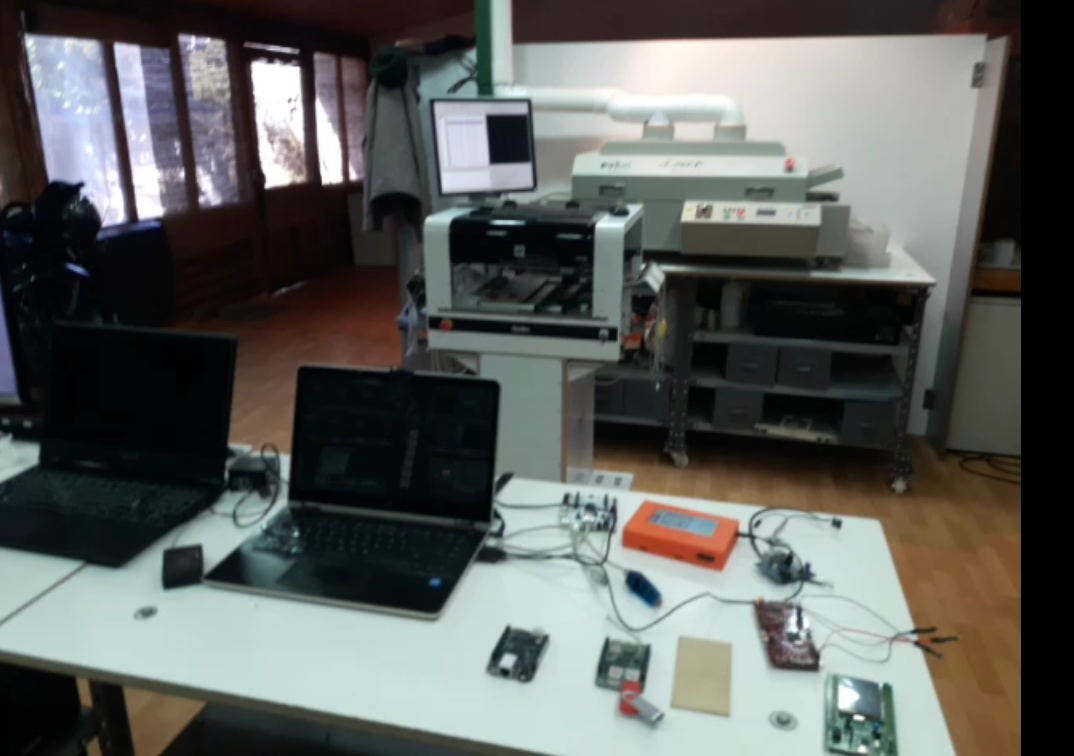
\includegraphics[width=0.3\textwidth]{ofi_dci2.png}
         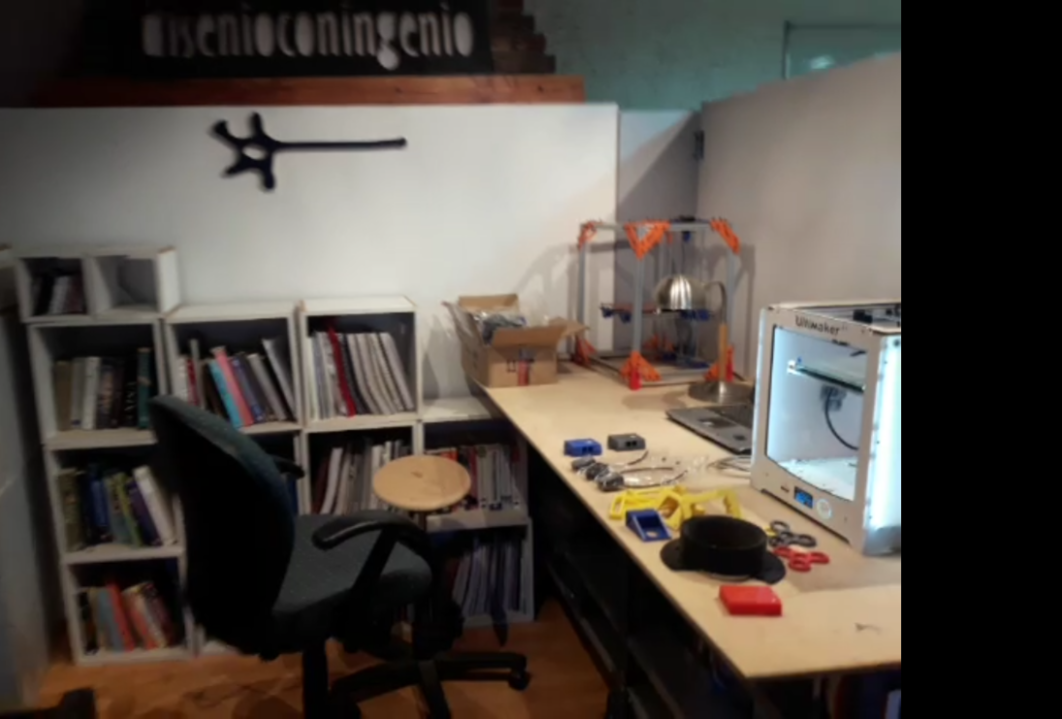
\includegraphics[width=0.3\textwidth]{ofi_dci5.png}
      \end{center}
      \caption{Laboratorio de desarrollo en Bariloche, 2019}
      \label{fig:ofi_dci}
   \end{figure}
\pagebreak


